\documentclass{article}
\usepackage{amsmath}
\usepackage{amssymb}
\usepackage{amsthm}
\usepackage{prooftree}
\usepackage{algorithm,algorithmic}
\usepackage{float}
\usepackage[svgnames]{xcolor}

% Proof rules and SOS rules.
\newcommand{\proofrule}[3][]{#1 \frac{\raisebox{.7ex}{\normalsize{$#2$}}}
  {\raisebox{-1.0ex}{\normalsize{$#3$}}}}

  % Modal equation systems
\newcommand{\E}{\mathcal{E}}
\newcommand{\eqmu}{\stackrel{\mu}{=}}
\newcommand{\eqnu}{\stackrel{\nu}{=}}
\newcommand{\eqsigma}{\stackrel{\sigma}{=}}
\newcommand{\lhs}{\mathsf{lhs}}
\newcommand{\rhs}{\mathsf{rhs}}

\newcommand{\placeholder}[1][]{\pi_{#1}}

\newcommand{\loc}{l}
\newcommand{\region}{\mathit{cc}}

\newcommand{\suc}{\mathit{succ}}
\newcommand{\pre}{\mathit{pred}}
\newcommand{\inv}{\mathit{inv}}
\newcommand{\post}{\mathit{post}}

\newcommand{\var}[1]{\ensuremath{\mathit{#1}}}
\newcommand{\method}[1]{\ensuremath{\mathbf{#1}}}
\newcommand{\true}{\texttt{true}}
\newcommand{\false}{\texttt{false}}

\usepackage[textwidth=3.2cm]{todonotes}
%\setlength{\marginparwidth}{3.2cm}
\newcommand{\jk}[2][]{\todo[#1]{JK: #2}}

\title{Implementation notes for TimeSolver}
\author{Jeroen J.A. Keiren}

\begin{document}

\maketitle


In this note we describe the proof rules as they are implemented in TimeSolver. We stick as close as possible to the implementation.
The rules were described originally in \cite{ZC:05rtss}, and the rules with placeholder stem from \cite{FC:14}. A more elaborate
discussion about (some of) the proof rules can be found in \cite{FC:14report}.

The proof rules are implemented in the file \texttt{proof.hh}. This is a header-only implementation to allow the compiler to inline wherever possible.
The class \texttt{prover} supports proof rules without placeholder, named \texttt{do\_proof\_*}, and proof rules with placeholder, named \texttt{do\_proof\_place\_*}. Note that the rules without placeholders can call the rules with placeholders, but not the other way around. The methods with placeholder correspond to those proof rules in which a placeholder is present in the goal.

Below we describe each of the proof rules as they are implemented in the tool.

\section{Helper functions}
Before we delve into the algorithms for each of the operators, we first look at some side conditions that need to be computed.

The first of these is a side condition that we will use, among others, for relativized exists. Given a region $(\loc, \region)$, placeholders $\placeholder[1], \placeholder[2] \subseteq \inv(\loc)$, we need to find the largest placeholder $\placeholder \subseteq \placeholder[2]$ such that $\suc((\loc, \region)) \cap \pre_{<}(\placeholder) \subseteq \suc((\loc, \region)) \cap \placeholder[1]$.

We first introduce the problem by considering the property $\exists_{x_1 \leq 3}(x_2 = 3)$, such that $\placeholder[1] \equiv x_1 \leq 3$, and $\placeholder[2] \equiv x_2 = 3$, and in which the clock region $(\loc, \region) \equiv 0 \leq x_1 \leq 2 \land 0 \leq x_2 \leq 1$.

First, observe that choosing $\placeholder \equiv \placeholder[2] \equiv x_2 = 3$ does not satisfy the conditions since $\pre_{<}(x_2 = 3) = x_2 < 3$, which includes states outside $x_1 \leq 3$. We show this in the following picture, where the relevant regions are shaded ($\placeholder[1]$ green, $\pre_{<}(\placeholder[2])$ blue, and $\suc((\loc, \region))$ red); $(\loc, \region)$ is the small rectangle at the bottom-left of the picture.

\begin{center}
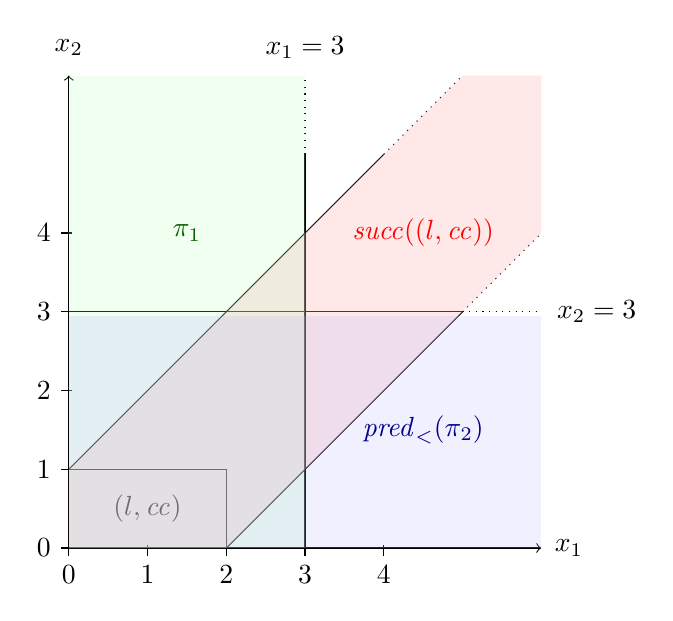
\begin{tikzpicture}
% axis
\draw[->] (0,0) -- (6, 0) coordinate (x axis);
\draw[->] (0, 0) -- (0, 6) coordinate (y axis);
% ticks
\foreach \x in {0,...,4,}
  \draw (\x,1pt) -- (\x,-3pt) node[anchor=north] {\x};
\foreach \y in {0,...,4}
  \draw (1pt,\y) -- (-3pt,\y) node[anchor=east] {\y}; 

% labels
\node[xshift=10pt] at (x axis) {$x_1$};
\node[yshift=10pt] at (y axis) {$x_2$};

% (l, cc)
\draw (0,0) rectangle (2,1);
\node at (1,0.5) {$(\loc, \region)$};

% (x_1 = 3)
\draw (3,0) -- (3,5);
\draw[dotted] (3,5) -- (3,6) coordinate (x1 label);
\node[yshift=10pt] at (x1 label) {$x_1 = 3$};

% (x_2 = 3)
\draw (0,3) -- (5,3);
\draw[dotted] (5,3) -- (6,3) coordinate (x2 label);
\node[xshift=20pt] at (x2 label) {$x_2 = 3$};

% succ((l,cc)) boundaries
\draw (0,1) -- (4,5)
      (2,0) -- (5,3);
\draw[dotted] (4,5) -- (5,6)
              (5,3) -- (6,4); 
% succ((l,cc)) shading
\draw[fill=red!30, fill opacity=0.3,draw=none] (0,0) -- (0,1) -- (5,6) -- (6,6) -- (6,4) -- (2,0);
\node[color=red] at (4.5,4) {$\suc((\loc, \region))$};

% placeholder 1
\draw[fill=green!30, fill opacity=0.2, draw=none] (0,0) rectangle (3,6);
\node[color=DarkGreen] at (1.5,4) {$\placeholder[1]$};

% pred_{<}(placeholder 2)
\draw[fill=blue!30, fill opacity=0.2, draw=none]
(0,0) rectangle (6,2.95);
\node[color=DarkBlue] at (4.5,1.5) {$\pre_{<}(\placeholder[2])$};

\end{tikzpicture}
\end{center}
In particular, the condition is not satisfied due to the triangle in which $\suc((\loc, \region))$ and $\pre_{<}(\placeholder[2])$ overlap, which is not included in $\placeholder[1]$. To eliminate this, we must restrict $\placeholder$ such that $\suc((\loc, \region)) \cap \pre_{<}(\placeholder)$ does not include this \emph{bad} triangle.

This bad region can be identified by $\mathit{bad} \equiv (\suc((\loc, \region)) \cap \pre_{<}(\placeholder[2])) \setminus \placeholder[1]$.
From this bad region we determine the states in $(\loc, \region)$ from which they can be reached using $(\loc, \region) \cap \pre(\mathit{bad})$.

\begin{center}
  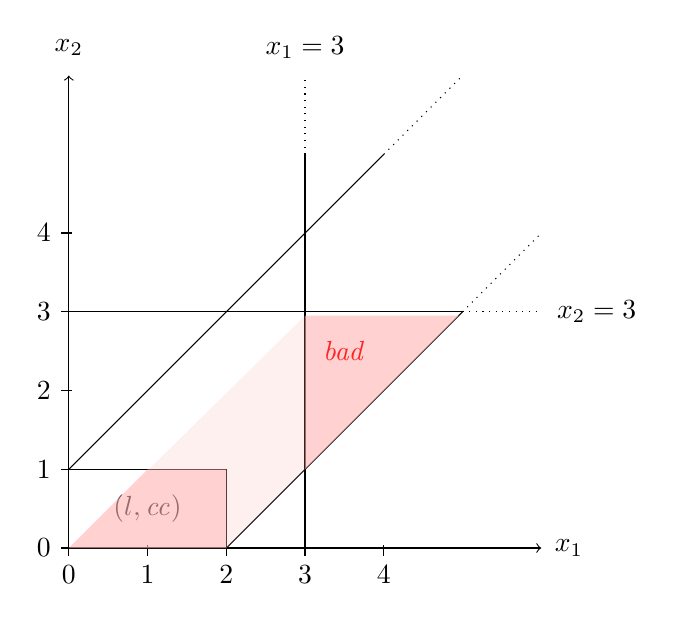
\begin{tikzpicture}
  % axis
  \draw[->] (0,0) -- (6, 0) coordinate (x axis);
  \draw[->] (0, 0) -- (0, 6) coordinate (y axis);
  % ticks
  \foreach \x in {0,...,4,}
    \draw (\x,1pt) -- (\x,-3pt) node[anchor=north] {\x};
  \foreach \y in {0,...,4}
    \draw (1pt,\y) -- (-3pt,\y) node[anchor=east] {\y}; 
  
  % labels
  \node[xshift=10pt] at (x axis) {$x_1$};
  \node[yshift=10pt] at (y axis) {$x_2$};
  
  % (l, cc)
  \draw (0,0) rectangle (2,1);
  \node at (1,0.5) {$(\loc, \region)$};
  
  % (x_1 = 3)
  \draw (3,0) -- (3,5);
  \draw[dotted] (3,5) -- (3,6) coordinate (x1 label);
  \node[yshift=10pt] at (x1 label) {$x_1 = 3$};
  
  % (x_2 = 3)
  \draw (0,3) -- (5,3);
  \draw[dotted] (5,3) -- (6,3) coordinate (x2 label);
  \node[xshift=20pt] at (x2 label) {$x_2 = 3$};
  
  % succ((l,cc)) boundaries
  \draw (0,1) -- (4,5)
        (2,0) -- (5,3);
  \draw[dotted] (4,5) -- (5,6)
                (5,3) -- (6,4); 
  % succ((l,cc)) shading
  %\draw[fill=red!30, fill opacity=0.3,draw=none] (0,0) -- (0,1) -- (5,6) -- (6,6) -- (6,4) -- (2,0);
  %\node[color=red] at (4.5,4) {$\suc((\loc, \region))$};
  
  % placeholder 1
  %\draw[fill=green!30, fill opacity=0.2, draw=none] (0,0) rectangle (3,6);
  %\node[color=DarkGreen] at (1.5,4) {$\placeholder[1]$};
  
  % pred_{<}(placeholder 2)
  %\draw[fill=blue!30, fill opacity=0.2, draw=none]
  %(0,0) rectangle (6,2.95);
  %\node[color=DarkBlue] at (4.5,1.5) {$\pre_{<}(\placeholder[2])$};
  
  % bad
  \draw[fill=red!30,draw=none,fill opacity=0.5] (3,1) -- (3,2.95) -- (4.95,2.95) -- (3,1);
  \node[color=red] at (3.5,2.5) {$\mathit{bad}$};
  \draw[fill=red!30,draw=none, fill opacity=0.5] (0,0) -- (1,1) -- (2,1) -- (2,0) -- (0,0);
  \draw[fill=red!30,draw=none, fill opacity=0.2] (0,0) -- (3,2.95) -- (4.95,2.95) -- (2,0) -- (0,0);
  
  
  \end{tikzpicture}
  \end{center}

To compute $\placeholder$ we need to remove those states from $\placeholder[2]$ that can be reached from $(\loc, \region) \cap \pre(\mathit{bad})$, which is $\placeholder[2] \setminus \suc((\loc, \region) \cap \pre(\mathit{bad})$. The bad part of $\placeholder[2]$
is indicated in red; the good part is indicated in blue in de the figure below.

\begin{center}
  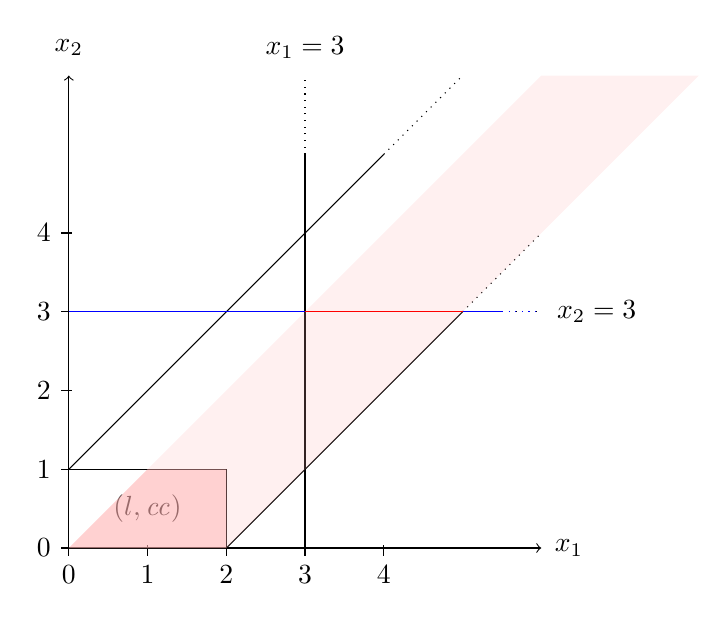
\begin{tikzpicture}
  % axis
  \draw[->] (0,0) -- (6, 0) coordinate (x axis);
  \draw[->] (0, 0) -- (0, 6) coordinate (y axis);
  % ticks
  \foreach \x in {0,...,4,}
    \draw (\x,1pt) -- (\x,-3pt) node[anchor=north] {\x};
  \foreach \y in {0,...,4}
    \draw (1pt,\y) -- (-3pt,\y) node[anchor=east] {\y}; 
  
  % labels
  \node[xshift=10pt] at (x axis) {$x_1$};
  \node[yshift=10pt] at (y axis) {$x_2$};
  
  % (l, cc)
  \draw (0,0) rectangle (2,1);
  \node at (1,0.5) {$(\loc, \region)$};
  
  % (x_1 = 3)
  \draw (3,0) -- (3,5);
  \draw[dotted] (3,5) -- (3,6) coordinate (x1 label);
  \node[yshift=10pt] at (x1 label) {$x_1 = 3$};
  
  % (x_2 = 3)
  \draw (0,3) -- (5,3);
  \draw[dotted] (5,3) -- (6,3) coordinate (x2 label);
  \node[xshift=20pt] at (x2 label) {$x_2 = 3$};
  
  % succ((l,cc)) boundaries
  \draw (0,1) -- (4,5)
        (2,0) -- (5,3);
  \draw[dotted] (4,5) -- (5,6)
                (5,3) -- (6,4); 
  % succ((l,cc)) shading
  %\draw[fill=red!30, fill opacity=0.3,draw=none] (0,0) -- (0,1) -- (5,6) -- (6,6) -- (6,4) -- (2,0);
  %\node[color=red] at (4.5,4) {$\suc((\loc, \region))$};
  
  % placeholder 1
  %\draw[fill=green!30, fill opacity=0.2, draw=none] (0,0) rectangle (3,6);
  %\node[color=DarkGreen] at (1.5,4) {$\placeholder[1]$};
  
  % pred_{<}(placeholder 2)
  %\draw[fill=blue!30, fill opacity=0.2, draw=none]
  %(0,0) rectangle (6,2.95);
  %\node[color=DarkBlue] at (4.5,1.5) {$\pre_{<}(\placeholder[2])$};
  
  % bad
  \draw[fill=red!30,draw=none, fill opacity=0.5] (0,0) -- (1,1) -- (2,1) -- (2,0) -- (0,0);
  \draw[fill=red!30,draw=none, fill opacity=0.2] (0,0) -- (6,6) -- (8,6) -- (2,0) -- (0,0);

  \draw[color=red] (3,3) -- (5,3);
  \draw[color=blue] (0,3) -- (3,3);
  \draw[color=blue] (5,3) -- (5.5,3);
  \draw[color=blue, dotted] (5.5,3) -- (6,3); 
  
  \end{tikzpicture}
  \end{center}

In order to fully satisfy the side condition, we still need to make sure that
$\pre_<(\placeholder) \subseteq \placeholder[1]$, which can be achieved by
intersecting the aforementioned region with $\placholder[1]$. The resulting value
of $\placeholder$ is thus $\placeholder \equiv (\placeholder[2] \setminus \suc((\loc, \region) \cap \pre(\mathit{bad})) \cap \placeholder[1]$. The resulting placeholder $\placeholder$ is indicated in the
following figure.
In the proof rule for relativized $\exists$, the value of $\placeholder[\exists]$
can be chosen such that $\placeholder[\exists] \equiv \pre(\placeholder)$. The
side condition $(\loc, \region) \cap \placeholder[\exists] \subseteq \pre(\placeholder)$
is then satisfied immediately. The shaded area in the following diagram gives
$\placeholder[\exists]$, $(\loc, \region) \cap \placeholder[\exists]$ is indicated
in a darker shade.

\begin{center}
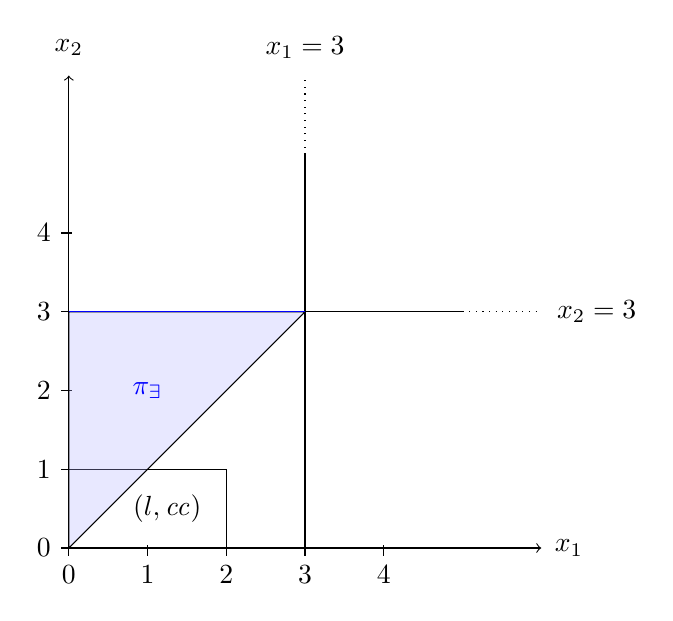
\begin{tikzpicture}
% axis
\draw[->] (0,0) -- (6, 0) coordinate (x axis);
\draw[->] (0, 0) -- (0, 6) coordinate (y axis);
% ticks
\foreach \x in {0,...,4,}
  \draw (\x,1pt) -- (\x,-3pt) node[anchor=north] {\x};
\foreach \y in {0,...,4}
  \draw (1pt,\y) -- (-3pt,\y) node[anchor=east] {\y}; 

% labels
\node[xshift=10pt] at (x axis) {$x_1$};
\node[yshift=10pt] at (y axis) {$x_2$};

% (l, cc)
\draw (0,0) rectangle (2,1);
\node at (1.25,0.5) {$(\loc, \region)$};

% (x_1 = 3)
\draw (3,0) -- (3,5);
\draw[dotted] (3,5) -- (3,6) coordinate (x1 label);
\node[yshift=10pt] at (x1 label) {$x_1 = 3$};

% (x_2 = 3)
\draw (0,3) -- (5,3);
\draw[dotted] (5,3) -- (6,3) coordinate (x2 label);
\node[xshift=20pt] at (x2 label) {$x_2 = 3$};

% % succ((l,cc)) boundaries
% \draw (0,1) -- (4,5)
%       (2,0) -- (5,3);
% \draw[dotted] (4,5) -- (5,6)
%               (5,3) -- (6,4); 
% % succ((l,cc)) shading
% \draw[fill=red!30, fill opacity=0.3,draw=none] (0,0) -- (0,1) -- (5,6) -- (6,6) -- (6,4) -- (2,0);
% \node[color=red] at (4.5,4) {$\suc((\loc, \region))$};

% resulting placeholder
\draw[fill=blue!30, fill opacity=0.3] (0,0) -- (0,3) -- (3,3) -- (0,0);
\node[color=blue] at (1,2) {$\placeholder[\exists]$};
\draw[color=blue] (0,3) -- (3,3);

% % succ((l,cc) \cap placeholder) boundaries
% \draw (0,1) -- (4,5)
%       (0,0) -- (4,4);ı
% \draw[dotted] (4,5) -- (5,6)
%                (4,4) -- (6,6); 
% % succ((l,cc) \cap \placeholder) shading
% \draw[fill=red!30, fill opacity=0.3,draw=none] (0,0) -- (0,1) -- (5,6) -- (6,6) -- (0,0);
% \node[color=red,rotate=45] at (3.5,4) {$\suc((\loc, \region) \cap \placeholder[\exists])$};

% % placeholder 1
% \draw[fill=green!30, fill opacity=0.2, draw=none] (0,0) rectangle (3,6);
% \node[color=DarkGreen] at (1.5,4) {$\placeholder[1]$};

% pred_{<}(placeholdeır 2)
% \draw[fill=blue!30, fill opacity=0.2, draw=none]
% (0,0) rectangle (6,2.95);
% \node[color=DarkBlue] at (4.5,1.5) {$\pre_{<}(\placeholder[2])$};

\end{tikzpicture}
\end{center}

\subsection{An additional example}

As an additional example, consider the property
 $\exists_{x_1 \leq 3}(x_2 = 2 \lor x_2 = 3)$, such that
 $\placeholder[1] \equiv x_1 \leq 3$, and $\placeholder[2] \equiv x_2 = 2 \lor 
 x_2 = 3$, and in which the clock region
 $(\loc, \region) \equiv 0 \leq x_1 \leq 2 \land 0 \leq x_2 \leq 1$.
 For the sake of conciseness let us write $\placeholder[2]^1 \equiv x_2 = 2$ and
 $\placeholder[2]^2 \equiv x_2 = 3$.

First, observe that choosing $\placeholder \equiv \placeholder[2]$
does not satisfy the conditions since $\pre_{<}(x_2 = 2 \lor x _2 = 3) = x_2 < 3$, which includes states outside $x_1 \leq 3$. We show this in the following picture,
where the relevant regions are shaded ($\placeholder[1]$ green, 
$\pre_{<}(\placeholder[2])$ blue, and $\suc((\loc, \region))$ red);
$(\loc, \region)$ is the small rectangle at the bottom-left of the picture.

\begin{center}
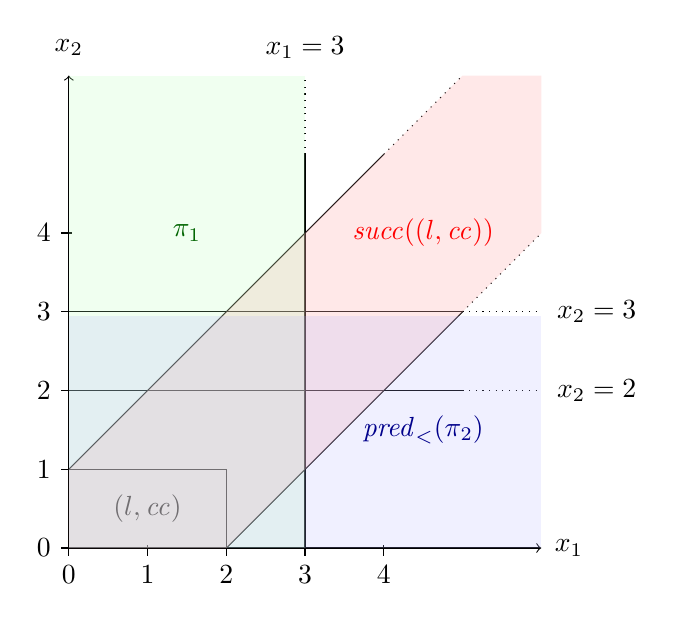
\begin{tikzpicture}
% axis
\draw[->] (0,0) -- (6, 0) coordinate (x axis);
\draw[->] (0, 0) -- (0, 6) coordinate (y axis);
% ticks
\foreach \x in {0,...,4,}
  \draw (\x,1pt) -- (\x,-3pt) node[anchor=north] {\x};
\foreach \y in {0,...,4}
  \draw (1pt,\y) -- (-3pt,\y) node[anchor=east] {\y}; 

% labels
\node[xshift=10pt] at (x axis) {$x_1$};
\node[yshift=10pt] at (y axis) {$x_2$};

% (l, cc)
\draw (0,0) rectangle (2,1);
\node at (1,0.5) {$(\loc, \region)$};

% (x_1 = 3)
\draw (3,0) -- (3,5);
\draw[dotted] (3,5) -- (3,6) coordinate (x1 label);
\node[yshift=10pt] at (x1 label) {$x_1 = 3$};

% (x_2 = 2)
\draw (0,2) -- (5,2);
\draw[dotted] (5,2) -- (6,2) coordinate (x2 label);
\node[xshift=20pt] at (x2 label) {$x_2 = 2$};

% (x_2 = 3)
\draw (0,3) -- (5,3);
\draw[dotted] (5,3) -- (6,3) coordinate (x2 label);
\node[xshift=20pt] at (x2 label) {$x_2 = 3$};

% succ((l,cc)) boundaries
\draw (0,1) -- (4,5)
      (2,0) -- (5,3);
\draw[dotted] (4,5) -- (5,6)
              (5,3) -- (6,4); 
% succ((l,cc)) shading
\draw[fill=red!30, fill opacity=0.3,draw=none] (0,0) -- (0,1) -- (5,6) -- (6,6) -- (6,4) -- (2,0);
\node[color=red] at (4.5,4) {$\suc((\loc, \region))$};

% placeholder 1
\draw[fill=green!30, fill opacity=0.2, draw=none] (0,0) rectangle (3,6);
\node[color=DarkGreen] at (1.5,4) {$\placeholder[1]$};

% pred_{<}(placeholder 2)
\draw[fill=blue!30, fill opacity=0.2, draw=none]
(0,0) rectangle (6,2.95);
\node[color=DarkBlue] at (4.5,1.5) {$\pre_{<}(\placeholder[2])$};

\end{tikzpicture}
\end{center}
In particular, the condition is not satisfied due to the triangle in which
$\suc((\loc, \region))$ and $\pre_{<}(\placeholder[2]^1)$ overlap, which is not included
in $\placeholder[1]$. To eliminate this, we must restrict $\placeholder$ such
that $\suc((\loc, \region)) \cap \pre_{<}(\placeholder)$ does not include this
\emph{bad} triangle.

Now, observe that, contrary to our previous example, we cannot identify this
bad region by choosing $\mathit{bad} \equiv (\suc((\loc, \region)) \cap
\pre_{<}(\placeholder[2])) \setminus \placeholder[1]$ (this would lead us to
identify the same bad region as in the previous example). This is due to the
placeholder not being convex. This can be overcome by treating the convex
parts of the placeholder separately. For the good part of the placeholder w.r.t.
$\placeholder[2]^2$ we refer to the exposition given previously. We here focus
on $\placeholder[2]^1 \equiv x_2 = 2$.

With respect to $x_2 = 2$, we can identify the bad region by choosing
$\mathit{bad}^1 \equiv (\suc((\loc, \region)) \cap
\pre_{<}(\placeholder[2]^1)) \setminus \placeholder[1]$. 
From this bad region we determine the states in $(\loc, \region)$ from which
they can be reached using $(\loc, \region) \cap \pre(\mathit{bad}^1)$.

\begin{center}
  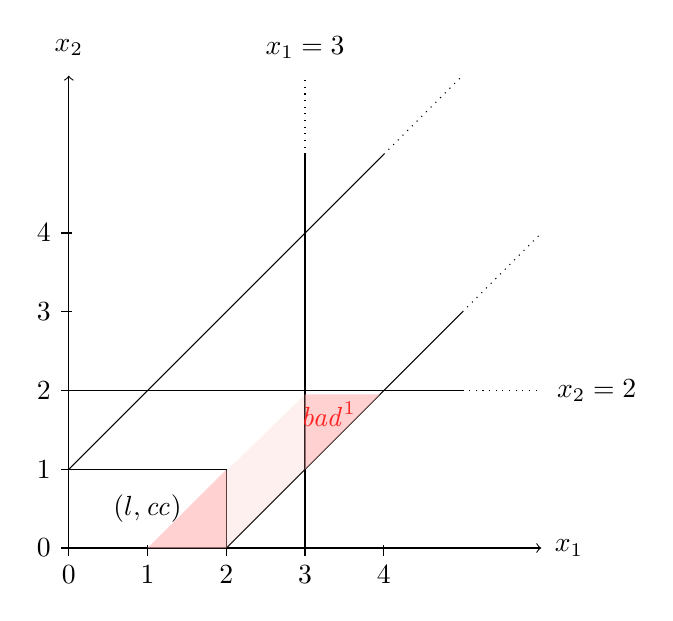
\begin{tikzpicture}
  % axis
  \draw[->] (0,0) -- (6, 0) coordinate (x axis);
  \draw[->] (0, 0) -- (0, 6) coordinate (y axis);
  % ticks
  \foreach \x in {0,...,4,}
    \draw (\x,1pt) -- (\x,-3pt) node[anchor=north] {\x};
  \foreach \y in {0,...,4}
    \draw (1pt,\y) -- (-3pt,\y) node[anchor=east] {\y}; 
  
  % labels
  \node[xshift=10pt] at (x axis) {$x_1$};
  \node[yshift=10pt] at (y axis) {$x_2$};
  
  % (l, cc)
  \draw (0,0) rectangle (2,1);
  \node at (1,0.5) {$(\loc, \region)$};
  
  % (x_1 = 3)
  \draw (3,0) -- (3,5);
  \draw[dotted] (3,5) -- (3,6) coordinate (x1 label);
  \node[yshift=10pt] at (x1 label) {$x_1 = 3$};
  
  % (x_2 = 2)
  \draw (0,2) -- (5,2);
  \draw[dotted] (5,2) -- (6,2) coordinate (x2 label);
  \node[xshift=20pt] at (x2 label) {$x_2 = 2$};
  
  % succ((l,cc)) boundaries
  \draw (0,1) -- (4,5)
        (2,0) -- (5,3);
  \draw[dotted] (4,5) -- (5,6)
                (5,3) -- (6,4); 
  % succ((l,cc)) shading
  %\draw[fill=red!30, fill opacity=0.3,draw=none] (0,0) -- (0,1) -- (5,6) -- (6,6) -- (6,4) -- (2,0);
  %\node[color=red] at (4.5,4) {$\suc((\loc, \region))$};
  
  % placeholder 1
  %\draw[fill=green!30, fill opacity=0.2, draw=none] (0,0) rectangle (3,6);
  %\node[color=DarkGreen] at (1.5,4) {$\placeholder[1]$};
  
  % pred_{<}(placeholder 2)
  %\draw[fill=blue!30, fill opacity=0.2, draw=none]
  %(0,0) rectangle (6,2.95);
  %\node[color=DarkBlue] at (4.5,1.5) {$\pre_{<}(\placeholder[2])$};
  
  % bad
  \draw[fill=red!30,draw=none,fill opacity=0.5] (3,1) -- (3,1.95) -- (3.95,1.95) -- (3,1);
  \node[color=red] at (3.3,1.7) {$\mathit{bad}^1$};
  \draw[fill=red!30,draw=none, fill opacity=0.5] (1,0) -- (2,1) -- (2,0) -- (1,0);
  \draw[fill=red!30,draw=none, fill opacity=0.2] (1,0) -- (3,1.95) -- (3.95,1.95) -- (2,0) -- (1,0);
  
  
  \end{tikzpicture}
  \end{center}

We need to remove those states from $\placeholder[2]^1$ that can be reached from 
$(\loc, \region) \cap \pre(\mathit{bad}^1)$, which is
$\placeholder[2]^1 \setminus \suc((\loc, \region) \cap \pre(\mathit{bad}^1)$.
The bad part of $\placholder[2]^1$ is indicated in red; the good part is indicated in
blue in de the figure below. Let us call the resulting placeholder $\placeholder^1$.

\begin{center}
  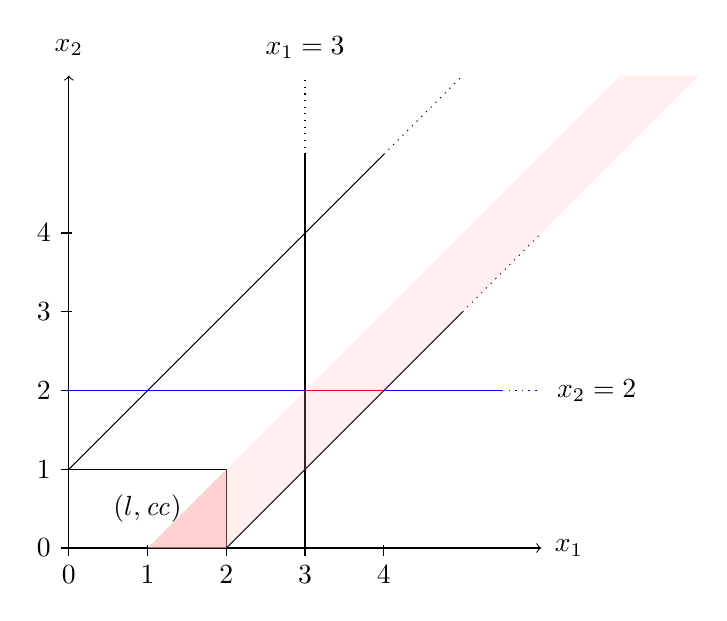
\begin{tikzpicture}
  % axis
  \draw[->] (0,0) -- (6, 0) coordinate (x axis);
  \draw[->] (0, 0) -- (0, 6) coordinate (y axis);
  % ticks
  \foreach \x in {0,...,4,}
    \draw (\x,1pt) -- (\x,-3pt) node[anchor=north] {\x};
  \foreach \y in {0,...,4}
    \draw (1pt,\y) -- (-3pt,\y) node[anchor=east] {\y}; 
  
  % labels
  \node[xshift=10pt] at (x axis) {$x_1$};
  \node[yshift=10pt] at (y axis) {$x_2$};
  
  % (l, cc)
  \draw (0,0) rectangle (2,1);
  \node at (1,0.5) {$(\loc, \region)$};
  
  % (x_1 = 3)
  \draw (3,0) -- (3,5);
  \draw[dotted] (3,5) -- (3,6) coordinate (x1 label);
  \node[yshift=10pt] at (x1 label) {$x_1 = 3$};
  
  % (x_2 = 3)
  \draw (0,2) -- (5,2);
  \draw[dotted] (5,2) -- (6,2) coordinate (x2 label);
  \node[xshift=20pt] at (x2 label) {$x_2 = 2$};
  
  % succ((l,cc)) boundaries
  \draw (0,1) -- (4,5)
        (2,0) -- (5,3);
  \draw[dotted] (4,5) -- (5,6)
                (5,3) -- (6,4); 
  % succ((l,cc)) shading
  %\draw[fill=red!30, fill opacity=0.3,draw=none] (0,0) -- (0,1) -- (5,6) -- (6,6) -- (6,4) -- (2,0);
  %\node[color=red] at (4.5,4) {$\suc((\loc, \region))$};
  
  % placeholder 1
  %\draw[fill=green!30, fill opacity=0.2, draw=none] (0,0) rectangle (3,6);
  %\node[color=DarkGreen] at (1.5,4) {$\placeholder[1]$};
  
  % pred_{<}(placeholder 2)
  %\draw[fill=blue!30, fill opacity=0.2, draw=none]
  %(0,0) rectangle (6,2.95);
  %\node[color=DarkBlue] at (4.5,1.5) {$\pre_{<}(\placeholder[2])$};
  
  % bad
  \draw[fill=red!30,draw=none, fill opacity=0.5] (1,0) -- (2,1) -- (2,0) -- (1,0);
  \draw[fill=red!30,draw=none, fill opacity=0.2] (1,0) -- (7,6) -- (8,6) -- (2,0) -- (1,0);

  \draw[color=red] (3,2) -- (4,2);
  \draw[color=blue] (0,2) -- (3,2);
  \draw[color=blue] (4,2) -- (5.5,2);
  \draw[color=blue, dotted] (5.5,2) -- (6,2); 
  
  \end{tikzpicture}
  \end{center}

In order to fully satisfy the side condition, we still need to make sure that
$\pre_<(\placeholder^1) \subseteq \placeholder[1]$, which can be achieved by
intersecting the aforementioned region with $\placeholder[1]$. The resulting value
of $\placeholder^1$ is thus $\placeholder^1 \equiv (\placeholder[2]^1 \setminus \suc((\loc, \region) \cap \pre(\mathit{bad}^1)) \cap \placeholder[1]$. 

Finally, we have to wonder about the value of $\placeholder$. Observe that
$\pre_{<}(\placeholder[2]^1 \lor \placeholder[2]^2) \equiv \pre_{<}(\placeholder[2]^1) \lor \pre_{<}(\placeholder[2]^2)$. Therefore, in particular, $\pre_{<}(\placeholder[2]^1) \lor \pre_{<}(\placeholder[2]^2) \subseteq \placeholder[1] \iff \pre_{<}(\placeholder[2]^1) \subseteq \placeholder[1] \land \pre_{<}(\placeholder[2]^2) \subseteq \placeholder[1]$.

Again, in the proof rule for relativized $\exists$, the value of $\placeholder[\exists]$
can be chosen such that $\placeholder[\exists] \equiv \pre(\placeholder)$. The
side condition $(\loc, \region) \cap \placeholder[\exists] \subseteq \pre(\placeholder)$
is then satisfied immediately. The shaded area in the following diagram gives
$\placeholder[\exists]$, $(\loc, \region) \cap \placeholder[\exists]$ is indicated
in a darker shade.

\begin{center}
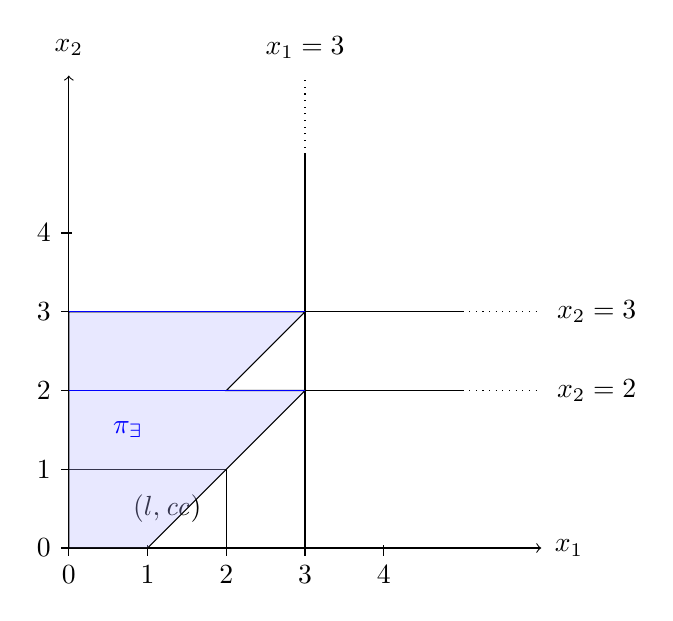
\begin{tikzpicture}
% axis
\draw[->] (0,0) -- (6, 0) coordinate (x axis);
\draw[->] (0, 0) -- (0, 6) coordinate (y axis);
% ticks
\foreach \x in {0,...,4,}
  \draw (\x,1pt) -- (\x,-3pt) node[anchor=north] {\x};
\foreach \y in {0,...,4}
  \draw (1pt,\y) -- (-3pt,\y) node[anchor=east] {\y}; 

% labels
\node[xshift=10pt] at (x axis) {$x_1$};
\node[yshift=10pt] at (y axis) {$x_2$};

% (l, cc)
\draw (0,0) rectangle (2,1);
\node at (1.25,0.5) {$(\loc, \region)$};

% (x_1 = 3)
\draw (3,0) -- (3,5);
\draw[dotted] (3,5) -- (3,6) coordinate (x1 label);
\node[yshift=10pt] at (x1 label) {$x_1 = 3$};

% (x_2 = 3)
\draw (0,3) -- (5,3);
\draw[dotted] (5,3) -- (6,3) coordinate (x2 label);
\node[xshift=20pt] at (x2 label) {$x_2 = 3$};

% (x_2 = 2)
\draw (0,2) -- (5,2);
\draw[dotted] (5,2) -- (6,2) coordinate (x2' label);
\node[xshift=20pt] at (x2' label) {$x_2 = 2$};

% % succ((l,cc)) boundaries
% \draw (0,1) -- (4,5)
%       (2,0) -- (5,3);
% \draw[dotted] (4,5) -- (5,6)
%               (5,3) -- (6,4); 
% % succ((l,cc)) shading
% \draw[fill=red!30, fill opacity=0.3,draw=none] (0,0) -- (0,1) -- (5,6) -- (6,6) -- (6,4) -- (2,0);
% \node[color=red] at (4.5,4) {$\suc((\loc, \region))$};

% resulting placeholder
\draw[fill=blue!30, fill opacity=0.3] (0,0) -- (0,3) -- (3,3) -- (2,2) -- (3,2) -- (1,0) -- (0,0);
\node[color=blue] at (.75,1.5) {$\placeholder[\exists]$};
\draw[color=blue] (0,3) -- (3,3);
\draw[color=blue] (0,2) -- (3,2);

% % succ((l,cc) \cap placeholder) boundaries
% \draw (0,1) -- (4,5)
%       (0,0) -- (4,4);ı
% \draw[dotted] (4,5) -- (5,6)
%                (4,4) -- (6,6); 
% % succ((l,cc) \cap \placeholder) shading
% \draw[fill=red!30, fill opacity=0.3,draw=none] (0,0) -- (0,1) -- (5,6) -- (6,6) -- (0,0);
% \node[color=red,rotate=45] at (3.5,4) {$\suc((\loc, \region) \cap \placeholder[\exists])$};

% % placeholder 1
% \draw[fill=green!30, fill opacity=0.2, draw=none] (0,0) rectangle (3,6);
% \node[color=DarkGreen] at (1.5,4) {$\placeholder[1]$};

% pred_{<}(placeholdeır 2)
% \draw[fill=blue!30, fill opacity=0.2, draw=none]
% (0,0) rectangle (6,2.95);
% \node[color=DarkBlue] at (4.5,1.5) {$\pre_{<}(\placeholder[2])$};

\end{tikzpicture}
\end{center}


\section{Predicate variables}
The cases where the proof goal is a predicate variable is handled by the rules \texttt{do\_proof\_predicate} and \texttt{do\_proof\_place\_predicate}.

\[
\proofrule
{(\loc, \region) \vdash X}
{(\loc, \region) \vdash \phi}
%
\quad
%
\proofrule
{(\loc, \region), \placeholder \vdash X}
{(\loc, \region), \placeholder \vdash \phi}
\]
Where $X \eqsigma \phi \in \E$ is an equation in the PES.

\jk{Describe how the caching and cycle detection works}


\section{Boolean operators}

\subsection{Conjunction}

\[
\proofrule[\land]
{(\loc, \region) \vdash \phi_1 \land \phi_2}
{(\loc, \region) \vdash \phi_1
\quad (\loc, \region) \vdash \phi_2}
\]

\begin{algorithm}[H]
\caption{$\method{do\_proof\_and}(\loc, \region, \phi_1 \land \phi_2)$}
\begin{algorithmic}
\STATE $\var{result} \gets \method{do\_proof}(\loc, \region, \phi_1)$
\IF{\var{result}}
  \STATE $\var{result} \gets \method{do\_proof}(\loc, \region, \phi_2)$
\ENDIF
\RETURN \var{result}
\end{algorithmic}
\end{algorithm}

The following rule, with placeholders, is not described explicitly in~\cite{FC:14,FC:14report}, we invent a new name for it. The description is straightforward.
\[
\proofrule[\land_p]
{(\loc, \region), \placeholder \vdash \phi_1 \land \phi_2}
{(\loc, \region), \placeholder[1] \vdash \phi_1
\quad (\loc, \region), \placeholder[2] \vdash \phi_2}
\placeholder = \placeholder[1] \cap \placeholder[2]
\]

\begin{algorithm}[H]
\caption{$\method{do\_proof\_place\_and}(\loc, \region, \placeholder, \phi_1 \land \phi_2)$}
\begin{algorithmic}
\STATE $\placeholder[1] \gets \infty$
\STATE $\method{do\_proof\_place}(\loc, \region, \placeholder[1], \phi_1)$
\STATE $\placeholder \gets \placeholder \cap \placeholder[1]$
\IF{$\placeholder = \emptyset$}
  \STATE $\placeholder[2] \gets \infty$
  \STATE $\method{do\_proof\_place}(\loc, \region, \placeholder[2] \phi_2)$
  \STATE $\placeholder \gets \placeholder \cap \placeholder[2]$
\ENDIF
\end{algorithmic}
\end{algorithm}
Note that if all proof methods simply restrict the placeholder, we could simplify this to the following code.
Currently, this leads to incorrect output of the tool!
\begin{algorithm}[H]
\caption{$\method{do\_proof\_place\_and}(\loc, \region, \placeholder, \phi_1 \land \phi_2)$}
\begin{algorithmic}
\STATE $\method{do\_proof\_place}(\loc, \region, \placeholder, \phi_1)$
\IF{$\placeholder = \emptyset$}
  \STATE $\method{do\_proof\_place}(\loc, \region, \placeholder \phi_2)$
\ENDIF
\end{algorithmic}
\end{algorithm}

\subsection{Disjunction}
The proof rules for $\lor$ given in \cite{FC:14} are the following.
\[
\proofrule[\lor_l]
{(\loc, \region) \vdash \phi_1 \lor \phi_2}
{(\loc, \region) \vdash \phi_1}
%
\quad
\proofrule[\lor_r]
{(\loc, \region) \vdash \phi_1 \lor \phi_2}
{(\loc, \region) \vdash \phi_2}
\quad
\proofrule[\lor_c]
{(\loc, \region) \vdash \phi_1 \lor \phi_2}
{(\loc, \region), \placeholder \vdash \phi_1
\quad
(\loc, \region), \lnot \placeholder \vdash \phi_2
}
\]

\[
\proofrule[\lor_s]
{(\loc, \region) \vdash \phi_1 \lor \phi_2}
{(\loc, \region), \placeholder[1] \vdash \phi_1
\quad (\loc, \region), \placeholder[2] \vdash \phi_2}
(\loc, \region) \subseteq \placeholder[1] \cup \placeholder[2]
\]

This is combined into the following code.
\begin{algorithm}[H]
\caption{$\method{do\_proof\_or}(\loc, \region, \phi_1 \lor \phi_2)$}
\begin{algorithmic}
\STATE $\placeholder[1] \gets \infty$
\STATE $\method{do\_proof\_place}(\loc, \region, \placeholder[1], \phi_1)$
\IF[Rule $\lor_r$]{$\placeholder[1] = \emptyset$}
  \STATE $\var{result} \gets \method{do\_proof}(\loc, \region, \phi_2)$
\ELSIF[Rule $\lor_l$]{$(\loc, \region) \subseteq \placeholder[1]$}
   \STATE $\var{result} \gets \true$
\ELSE[Rule $\lor_s$]
  \STATE $\placeholder[2] = \infty$
  \STATE $\method{do\_proof\_place}(\loc, \region, \placeholder[2], \phi_2)$
  \STATE $\var{result} \gets (l,cc) \subseteq \placeholder[1] \cup \placeholder[2]$
\ENDIF
\RETURN \var{result}
\end{algorithmic}
\end{algorithm}

The tool also implements a ``simple or'' operator which can always be proven using the $\lor_l$ and $\lor_r$ rules.

\begin{algorithm}[H]
\caption{$\method{do\_proof\_or\_simple}(\loc, \region, \phi_1 \lor \phi_2)$}
\begin{algorithmic}
\STATE $\var{result} \gets \method{do\_proof}(\loc, \region, \phi_1)$
\COMMENT{Try rule $\lor_l$ first}
\IF[Rule $\lor_r$]{$\lnot \var{result}$}
  \STATE $\var{result} \gets \method{do\_proof}(\loc, \region, \phi_2)$
\ENDIF
\RETURN \var{result}
\end{algorithmic}
\end{algorithm}

With placeholders, we get the following proof rule, which generalised $\lor_s$. Note this is not given in
\cite{FC:14,FC:14report}.
\[
\proofrule[\lor_{s_2}]
{(\loc, \region), \placeholder \vdash \phi_1 \lor \phi_2}
{(\loc, \region), \placeholder[1] \vdash \phi_1
\quad (\loc, \region), \placeholder[2] \vdash \phi_2}
(\loc, \region) \cap \placeholder \subseteq \placeholder[1] \cup \placeholder[2]
\]
This sidecondition can be validated by ensuring $\placeholder \subseteq \placeholder[1] \cup \placeholder[2]$.

This gives rise to the following code.
\begin{algorithm}[H]
\caption{$\method{do\_proof\_place\_or}(\loc, \region, \placeholder, \phi_1 \lor \phi_2)$}
\begin{algorithmic}
\STATE $\placeholder[1] \gets \placeholder$
\STATE $\method{do\_proof\_place}(\loc, \region, \placeholder[1], \phi_1)$
\IF[First subgoal does not yet cover the entire placeholder]{$\placeholder[1] \neq \placeholder$}
  \STATE $\placeholder[2] = \placeholder$
  \STATE $\method{do\_proof\_place}(\loc, \region, \placeholder[2], \phi_2)$
  \STATE $\placeholder \gets \placeholder[1] \cup \placeholder[2]$
\ENDIF
\end{algorithmic}
\end{algorithm}

Again the case for simple or is considered separately. The language construct appears to be such that
the placeholder will always either be completely empty, or completely full.
\begin{algorithm}[H]
\caption{$\method{do\_proof\_place\_or\_simple}(\loc, \region, \placeholder, \phi_1 \lor \phi_2)$}
\begin{algorithmic}
\STATE $\placeholder[1] \gets \placeholder$
\STATE $\method{do\_proof\_place}(\loc, \region, \placeholder[1], \phi_1)$
\IF{$\placeholder[1] = \placeholder$}
  \STATE $\placeholder \gets \placeholder[1]$
\ELSE
  \STATE $\method{do\_proof\_place}(\loc, \region, \placeholder, \phi_2)$
\ENDIF
\end{algorithmic}
\end{algorithm}

\subsection{Exists}

\[
\proofrule[\exists_{t_1}]
{(\loc, \region) \vdash \exists(\phi)}
{\suc((\loc, \region)), \placeholder \vdash \phi}
(\loc, \region) \subseteq \pre(\placeholder)
\]
%
For $\exists(\phi)$ we need to ensure that we only consider valid time advances (those satisfying the invariants).
We therefore consider $\exists(\inv(\loc) \land \phi)$ instead.
We get the following derivation (which is given in \cite[Appendix C.2]{FC:14}.
\[
\proofrule[\exists_{t_1}]
{(\loc, \region) \vdash \exists(\inv(\loc) \land \phi)}
{
  \proofrule[\land_p]
  {\suc((\loc, \region)), \placeholder \vdash \inv(\loc) \land \phi}
  {\suc((\loc, \region)), \placeholder[1] \vdash \inv(\loc)
  \quad \suc((\loc, \region)), \placeholder[2] \vdash \phi}
  \placeholder = \placeholder[1] \cap \placeholder[2]
}
(\loc, \region) \subseteq \pre(\placeholder)
\]
The subgoal involving $\inv(\loc)$ can be proven setting $\placeholder[1] = \inv(\loc)$, which is
the most liberal placeholder to prove the subgoal. If we take this simplification, this forces $\placeholder[2] \subseteq \inv(\loc)$,
and we get the following proof rule (writing $\placeholder$ instead of $\placeholder[2]$).
\[
\proofrule
{(\loc, \region) \vdash \exists(\inv(\loc) \land \phi)}
{\suc((\loc, \region)), \placeholder \vdash \phi}
\begin{array}{l}
\placeholder \subseteq \inv(\loc) \\
(\loc, \region) \subseteq \pre(\placeholder)
\end{array}
\]

This is implemented in the following pseudocode. Note that this assumes the recursive
call to \method{do\_proof} only restricts the placeholder, and does not enlarge it.

\begin{algorithm}[H]
\caption{$\method{do\_proof\_exists}(\loc, \region, \exists(\phi))$}
\begin{algorithmic}
\STATE $\placeholder \gets \inv(\loc)$ \COMMENT{Rule $\exists_{t_1}$}
\STATE $\method{do\_proof\_place}(\loc, \suc(\region), \placeholder, \phi)$
\RETURN $\region \subseteq \pre(\placeholder)$
\end{algorithmic}
\end{algorithm}

\[
%
\proofrule[\exists_{t_2}]
{(\loc, \region), \placeholder[\exists] \vdash \exists(\phi)}
{\suc((\loc, \region)), \placeholder \vdash \phi}
\placeholder[\exists] \subseteq \pre(\placeholder)
\]

If we add the placeholder to the proof rule, we have a similar modification as
before. If we again do the derivation from \cite[Appendix C.2]{FC:14report} we get:
\[
\proofrule[\exists_{t_2}]
{(\loc, \region), \placeholder[\exists] \vdash \exists(\inv(\loc) \land \phi)}
{\proofrule[\land_p]
  {\suc((\loc, \region)), \placeholder \vdash \inv(\loc) \land \phi}
  {\suc((\loc, \region)), \placeholder[1] \vdash \inv(\loc)
   \quad \suc((\loc, \region)), \placeholder[2] \vdash \phi}
  \placeholder = \placeholder[1] \cap \placeholder[2]
}
(\loc, \region) \cap \placeholder[\exists] \subseteq \pre(\placeholder)
\]
We can again set $\placeholder[1] = \inv(\loc)$ to get rid of the first subgoal of the $\land$,
obtaining the following proof.
\[
\proofrule[\exists_{t_2}]
{(\loc, \region), \placeholder[\exists] \vdash \exists(\inv(\loc) \land \phi)}
{\suc((\loc, \region)), \placeholder \vdash \phi}
\begin{array}{l}
\placeholder \subseteq \inv(l)\\
(\loc, \region) \cap \placeholder[\exists] \subseteq \pre(\placeholder)
\end{array}
\]
The second side condition can be ensured immediately by ensuring $\placeholder[\exists] \subseteq \pre(\placeholder)$.

\begin{algorithm}[H]
\caption{$\method{do\_proof\_exists\_place}(\loc, \region, \placeholder[\exists], \exists(\phi))$}
\begin{algorithmic}
\STATE $\placeholder \gets \inv(\loc)$ \COMMENT{Rule $\exists_{t_2}$}
\STATE $\method{do\_proof\_place}(\loc, \suc(\region), \placeholder, \phi)$
\STATE $\placeholder[\exists] \gets \placeholder[\exists] \cap \pre(\placeholder)$
\end{algorithmic}
\end{algorithm}

% \[
% \proofrule[\exists_{t_1}-Inv]
% {(\loc, \region) \vdash \exists(\inv(\loc) \land \phi)}
% {\suc((\loc, \region)), \placeholder \vdash \inv(\loc)
% \quad \suc((\loc, \region)), \placeholder \vdash \phi}
% (\loc, \region) \subseteq \pre(\placeholder)
% %
% \quad
% %
% \proofrule[\exists_{t_2}]
% {(\loc, \region), \placeholder[\exists] \vdash \exists(\phi)}
% {\suc((\loc, \region)), \placeholder \vdash \phi}
% \placeholder[\exists] \subseteq \pre(\placeholder)
% \]

For relativized $\exists$ we have the following proof rule.
\[
\proofrule[\exists_{r_1}]
{(\loc, \region) \vdash \exists_{\phi_1}(\phi_2)}
{\suc((\loc,\region)), \placeholder[2] \vdash \phi_2
\quad
\suc((\loc, \region)), \pre_{<}(\placeholder[2]) \vdash \phi_1
}
(\loc, \region) \subseteq \pre(\placeholder[2])
\]

Note that here we also need to incorporate the invariant into the proof rule. We therefore
need to prove that $\exists_{(\inv(\loc) \land \phi_1)}(\inv(\loc) \land \phi_2)$ instead.
\[
\proofrule[\exists_{r_1}]
{(\loc, \region) \vdash \exists_{\inv(\loc) \land \phi_1}(\inv(\loc) \land \phi_2)}
{\suc((\loc,\region)), \placeholder[2] \vdash \inv(\loc) \land \phi_2
\quad
\suc((\loc, \region)), \pre_{<}(\placeholder[2]) \vdash \inv(\loc) \land \phi_1
}
(\loc, \region) \subseteq \pre(\placeholder[2])
\]

For the first subgoal, we have the following derivation.
\[
\proofrule[\land_p]
{\suc((\loc,\region)), \placeholder[2] \vdash \inv(\loc) \land \phi_2}
{\suc((\loc,\region)), \placeholder[2,1] \vdash \inv(\loc)
\quad \suc((\loc,\region)), \placeholder[2,2] \vdash \phi_2}
\placeholder[2] = \placeholder[2,1] \cap \placeholder[2,2]
\]
In this proof we can set $\placeholder[2,1] = \inv(\loc)$, if we simplify we obtain the following.
\[
\proofrule[\land_p]
{\suc((\loc,\region)), \placeholder[2] \vdash \inv(\loc) \land \phi_2}
{\suc((\loc,\region)), \placeholder[2,2] \vdash \phi_2}
\placeholder[2] = \inv(\loc) \cap \placeholder[2,2]
\]

For te second subgoal, we first replace $\pre_{<}(\placeholder[2])$ with a fresh
placeholder $\placeholder[1]$, and require $\suc((\loc, \region)) \cap \pre_{<}(\placeholder[2]) \subseteq \suc((\loc, \region)) \cap \placeholder[1]$.
Subsequently we apply the $\land_p$ rule.
\[
\proofrule
{\suc((\loc, \region)), \pre_{<}(\placeholder[2]) \vdash \inv(\loc) \land \phi_1}
{\proofrule[\land_p]
  {\suc((\loc, \region)), \placeholder[1] \vdash \inv(\loc) \land \phi_1}
  {\suc((\loc, \region)), \placeholder[1,1] \vdash \inv(\loc)
  \quad \suc((\loc, \region)), \placeholder[1,2] \vdash \phi_1}
  \placeholder[1] = \placeholder[1,1] \cap \placeholder[1,2]
}
\suc((\loc, \region)) \cap \pre_{<}(\placeholder[2]) \subseteq \suc((\loc, \region)) \cap \placeholder[1]
\]
We can again set $\placeholder[1,1] = \inv(\loc)$, and simplifying we obtain
\[
\proofrule
{\suc((\loc, \region)), \pre_{<}(\placeholder[2]) \vdash \inv(\loc) \land \phi_1}
{\suc((\loc, \region)), \placeholder[1,2] \vdash \phi_1}
\suc((\loc, \region)) \cap \pre_{<}(\placeholder[2]) \subseteq \suc((\loc, \region)) \cap \inv(\loc) \cap \placeholder[1,2]
\]
%
If we combine all of this, we get the following derived proof rule for relativized~$\exists$.
\[
\proofrule
{(\loc, \region) \vdash \exists_{\inv(\loc) \land \phi_1}(\inv(\loc) \land \phi_2)}
{\suc((\loc,\region)), \placeholder[2,2] \vdash \phi_2
\quad \suc((\loc, \region)), \placeholder[1,2] \vdash \phi_1
\quad }
\begin{array}{l}
(\loc, \region) \subseteq \pre(\placeholder[2]) \\
\placeholder[2] = \inv(\loc) \cap \placeholder[2,2] \\
\placeholder[1] = \inv(\loc) \cap \placeholder[1,2] \\
\suc((\loc, \region)) \cap \pre_{<}(\placeholder[2]) \subseteq \suc((\loc, \region)) \cap \placeholder[1]
\end{array}
\]

Finally, we incorporate the assumption that invariants are \emph{past closed}, we therefore get that $\pre_{<}(\placeholder[2]) \subseteq \placeholder[1]$ iff $\pre_{<}(\placeholder[2]) \subseteq \placeholder[1,2]$. We simplify to the following.
\[
\proofrule
{(\loc, \region) \vdash \exists_{\inv(\loc) \land \phi_1}(\inv(\loc) \land \phi_2)}
{\suc((\loc,\region)), \placeholder[2] \vdash \phi_2
\quad \suc((\loc, \region)), \placeholder[1] \vdash \phi_1
}
\begin{array}{l}
(\loc, \region) \subseteq \pre(\placeholder[2]) \\
\placeholder[1] \subseteq \inv(\loc) \\
\placeholder[2] \subseteq \inv(\loc) \\
\suc((\loc, \region)) \cap \pre_{<}(\placeholder[2]) \subseteq \suc((\loc, \region)) \cap \placeholder[1]
\end{array}
\]
Note that if $\placeholder[1] = \emptyset$, the property can still hold if $\phi_2$ is satisfied immediately (so $\pre_{<}(\placeholder[2]) = \emptyset$). This gives rise to the following pseudocode.

\begin{algorithm}[H]
\caption{$\method{do\_proof\_exists\_rel}(\loc, \region, \exists_{\phi_1}(\phi_2))$}
\begin{algorithmic}
\STATE $\placeholder[2] \gets \inv(\loc)$ \COMMENT{Rule $\exists_{r_1}$}
\STATE $\method{do\_proof\_place}(\loc, \suc(\region), \placeholder[2], \phi_2)$
\IF[First subgoal fails]{$\placeholder[2] = \emptyset$}
  \STATE $\var{result} \gets \false$
\ELSE[Solve second subgoal and check side conditions]
  \STATE $\placeholder[1] \gets \infty$
  \STATE $\method{do\_proof\_place}(\loc, \suc(\region), \placeholder[1], \phi_1)$
  \IF[$\phi_2$ needs to hold immediately]{$\placeholder[1] \cap \pre_{<}(\placeholder[2]) = \emptyset$}
    \STATE $\var{result} \gets \region \subseteq \placeholder[2]$
    % \STATE $\placeholder[2] \gets \placeholder[2] \cap \region$
    % \IF{$\placeholder[2] = \emptyset$}
    %   \STATE $\var{result} \gets \false$
    % \ELSE
    %   \STATE $\var{result} \gets \region \subseteq \placeholder[2]$
    % \ENDIF
  \ELSE[Check the side conditions]
    \STATE Let $\placeholder$ be such that $\placeholder \subseteq \placeholder[2]$, and
    $\pre_{<}(\placeholder) \subseteq \placeholder[1]$ if such $\placeholder$ exists, en $\placeholder = \emptyset$ otherwise.
    \STATE $\var{result} \gets \region \subseteq \pre(\placeholder)$
  \ENDIF
\ENDIF
\RETURN $\var{result}$
\end{algorithmic}
\end{algorithm}
 \todo{Check the inner else carefully, I believe this is what the implementation does in predCheckRule.}

If we incorporate the placeholder, we get the following proof rule.

\[
\proofrule[\exists_{r_2}]
{(\loc, \region), \placeholder[\exists] \vdash \exists_{\phi_1}(\phi_2)}
{\suc((\loc,\region)), \placeholder[2] \vdash \phi_2
\quad
\suc((\loc, \region)), \pre_{<}(\placeholder[2]) \vdash \phi_1
}
(\loc, \region) \cap \placeholder[\exists] \subseteq \pre(\placeholder[2])
\]

We again incorporate the invariant, to obtain the following.

\[
\proofrule[\exists_{r_2}]
{(\loc, \region), \placeholder[\exists] \vdash \exists_{\inv(\loc) \land \phi_1}(\inv(\loc) \land \phi_2)}
{\suc((\loc,\region)), \placeholder[2] \vdash \inv(\loc) \land \phi_2
\quad
\suc((\loc, \region)), \pre_{<}(\placeholder[2]) \vdash \inv(\loc) \land \phi_1
}
(\loc, \region) \cap \placeholder[\exists] \subseteq \pre(\placeholder[2])
\]

The derivations for the two subgoals are the same as before, only the side condition is different. We get the following proof rule.
\[
\proofrule[\exists_{r_2}]
{(\loc, \region), \placeholder[\exists] \vdash \exists_{\inv(\loc) \land \phi_1}(\inv(\loc) \land \phi_2)}
{\suc((\loc,\region)), \placeholder[2] \vdash \phi_2
\quad \suc((\loc, \region)), \placeholder[1] \vdash \phi_1
}
\begin{array}{l}
(\loc, \region) \cap \placeholder[\exists] \subseteq \pre(\placeholder[2]) \\
\placeholder[1] \subseteq \inv(\loc) \\
\placeholder[2] \subseteq \inv(\loc) \\
\suc((\loc, \region)) \cap \pre_{<}(\placeholder[2]) \subseteq \suc((\loc, \region)) \cap \placeholder[1]
\end{array}
\]
The first side condition can easily be validated by setting $\placeholder[\exists] = \pre(\placeholder[2])$.

\begin{algorithm}[H]
\caption{$\method{do\_proof\_place\_exists\_rel}(\loc, \region, \placeholder[\exists], \exists_{\phi_1}(\phi_2))$}
\begin{algorithmic}
\STATE $\placeholder[2] \gets \inv(\loc)$ \COMMENT{Rule $\exists_{r_1}$}
\STATE $\method{do\_proof\_place}(\loc, \suc(\region), \placeholder[2], \phi_2)$
\IF[First subgoal fails]{$\placeholder[2] = \emptyset$}
  \STATE $\placeholder[\exists] \gets \emptyset$
\ELSE[Solve second subgoal and check side conditions]
  \STATE $\placeholder[1] \gets \infty$
  \STATE $\method{do\_proof\_place}(\loc, \suc(\region), \placeholder[1], \phi_1)$
  \IF[$\phi_2$ needs to hold immediately]{$\placeholder[1] \cap \pre_{<}(\placeholder[2]) = \emptyset$}
    \STATE $\placeholder[\exists] \gets \region \cap \placeholder[2]$
  \ELSE[Check the side conditions]
    \STATE Let $\placeholder$ be such that $\placeholder \subseteq \placeholder[2]$, and
    $\pre_{<}(\placeholder) \subseteq \placeholder[1]$ if such $\placeholder$ exists, en $\placeholder = \emptyset$ otherwise.
    \STATE $\placeholder[\exists] \gets \placeholder[\exists] \cap \pre(\placeholder)$
  \ENDIF
\ENDIF
\end{algorithmic}
\end{algorithm}



Note that this pseudocode assumes we can find $\placeholder$ such that 
$\placeholder \subseteq \placeholder[2]$, and
$\pre_{<}(\placeholder) \subseteq \placeholder[1]$ if such $\placeholder$ exists,
and $\placeholder = \emptyset$ otherwise.

{\color{red} NOTE: we need to ensure that the placeholder can be reached, so we in fact need to
check $\suc((\loc, \region)) \cap \pre_{<}(\placeholder) \subseteq \suc((\loc, \region)) \cap \placeholder[1]$.}

Given $\placeholder[1] \subseteq \inv(\loc)$, $\placeholder[2] \subseteq \inv(\loc)$, we need to find $\placeholder \subseteq \placeholder[2]$ such that
$\suc((\loc, \region)) \cap \pre_{<}(\placeholder) \subseteq \suc((\loc, \region)) \cap \placeholder[1]$.

Observe that we can decide whether $\placeholder[2]$ satisfies this side condition by checking $\suc((\loc, \region)) \cap \pre_{<}(\placeholder[2]) \cap \overline{\suc((\loc, \region)) \cap \placeholder[1]} = \emptyset$.

\subsection{Forall}

The forall rule without placeholder is described as follows.
\[
\proofrule[\forall_{t_1}]
{(\loc, \region) \vdash \forall(\phi)}
{\suc((\loc, \region)) \vdash \phi}
\]

In the implementation, care needs to be taken that only the valid time successors of $\region$ are considered,
i.e., only thos time successors of $\region$ are considered that satisfy $\inv(\loc)$. To achieve this,
instead of $\forall(\phi)$, the invariant is incorporated, and the formula $\forall(\inv(\loc) \implies \phi)$
is proven. Note this formula is simplified to $\forall(\lnot \inv(\loc) \lor \phi)$.
We can now derive the following, using our rules:
\[
\proofrule[\forall_{t_1}]
{(\loc, \region) \vdash \forall(\lnot \inv(\loc) \lor \phi)}
{
\proofrule[*]{\suc((\loc, \region)) \vdash \lnot \inv(\loc) \lor \phi}
{\suc((\loc, \region)) \cap \inv(\loc) \vdash \phi
}
}
\]
where at $*$ we used the fact that $a \vdash \lnot b \lor c$ can be interpreted as
$a \implies (\lnot b \lor c)$, which is equivalent to $(a \land b) \implies c$.

The following implementation for $\forall(\phi)$ is now obtained.
\begin{algorithm}[H]
\caption{$\method{do\_proof\_forall}(\loc, \region, \forall(\phi))$}
\begin{algorithmic}
\RETURN $\method{do\_proof}(\loc, \suc(\region) \cap \inv(\loc), \phi)$
\end{algorithmic}
\end{algorithm}

The case of $\forall$ with placeholders is described using the following rule.
\[
\proofrule[\forall_{t_2}]
{(\loc, \region), \placeholder[\forall] \vdash \forall(\phi)}
{\suc((\loc, \region)), \placeholder \vdash \phi}
\suc((\loc, \region) \cap \placeholder[\forall]) \subseteq \suc((\loc, \region)) \land \placeholder
\]

Here we again need to incorporate the invariant, so we again look at applying the rule
to $\forall(\lnot \inv(\loc) \lor \phi)$ instead.
\[
\proofrule[\forall_{t_2}]
{(\loc, \region), \placeholder[\forall] \vdash \forall(\lnot \inv(\loc) \lor \phi)}
{
  \proofrule[\lor_{s_2}]
  {\suc((\loc, \region)), \placeholder \vdash \lnot \inv(\loc) \lor  \phi}
  {\suc((\loc, \region)), \placeholder[1] \vdash \lnot \inv(\loc)
    \quad \suc((\loc, \region)), \placeholder[2] \vdash \phi}
    \suc((\loc, \region)) \cap \placeholder \subseteq \placeholder[1] \cup \placeholder[2]
}
\begin{array}{l}
\suc((\loc, \region) \cap \placeholder[\forall])\\
\quad \subseteq \suc((\loc, \region)) \land \placeholder
\end{array}
\]

Here we can again set $\placeholder[1] = \lnot \inv(\loc)$. If we fill this in, we get
\[
\proofrule[\forall_{t_2}]
{(\loc, \region), \placeholder[\forall] \vdash \forall(\lnot \inv(\loc) \lor \phi)}
{
  \proofrule[\lor_{s_2}]
  {\suc((\loc, \region)), \placeholder \vdash \lnot \inv(\loc) \lor  \phi}
  {\suc((\loc, \region)), \placeholder[2] \vdash \phi}
    \suc((\loc, \region)) \cap \placeholder \subseteq \lnot \inv(\loc) \cup \placeholder[2]
}
\begin{array}{l}
\suc((\loc, \region) \cap \placeholder[\forall])\\
\quad \subseteq \suc((\loc, \region)) \land \placeholder
\end{array}
\]

This gives rise to the following pseudocode.
\begin{algorithm}[H]
\caption{$\method{do\_proof\_place\_forall}(\loc, \region, \placeholder[\forall], \forall(\phi))$}
\begin{algorithmic}
\STATE $\placeholder[2] \gets \infty$
\STATE $\method{do\_proof\_place}(\loc, \suc(\region), \placeholder[2], \phi)$
\IF{$\placeholder[2] = \emptyset$}
  \STATE $\placeholder[\forall] = \emptyset$
\ELSE
  \STATE Let $\placeholder[\forall]$ be such that 
  $\suc((\loc, \region) \cap \placeholder[\forall]) \quad \subseteq \suc((\loc, \region)) \land \placeholder$
  and $\suc((\loc, \region)) \cap \placeholder \subseteq \lnot \inv(\loc) \cup \placeholder[2]$
\ENDIF
\end{algorithmic}
\end{algorithm}

Now let us consider relativized forall. The actual proof rules are derived using \cite[Lemma 1]{FC:14}, which states that $\forall_{\phi_1}(\phi_2) = \forall(\phi_2) \lor \exists_{\phi_2}(\phi_1 \land \phi_2)$.
% \[
% \proofrule[\text{Lemma 1 (i)}]
% {(\loc, \region) \vdash \forall_{\phi_1}(\phi_2)}
% {(\loc, \region) \vdash \forall(\phi_2)}
% \quad
% \proofrule[\text{Lemma 1 (ii)}]
% {(\loc, \region) \vdash \forall_{\phi_1}(\phi_2)}
% {(\loc, \region) \vdash \exists_{\phi_2}(\phi_1 \land \phi_2)}
% \]

The first disjunct of the lemma directly induces proof rule $\forall_{ro_1}$.

For the second disjunct, we first derive a simplified proof using the proof rules for relativized
exists, analogous to the
derivation in \cite[Appendix C.1]{FC:14report}.
\[
\proofrule[\exists_{r_2}]
{(\loc, \region), \placeholder[\exists] \vdash \exists_{\phi_2}(\phi_1 \land \phi_2)}
{ {\proofrule[\land_p]
  {\suc((\loc, \region)), \placeholder[2] \vdash \phi_1 \land \phi_2}
  {\suc((\loc, \region)), \placeholder[2,1] \vdash \phi_1
    \quad \suc((\loc, \region)), \placeholder[2,2] \vdash \phi_2}
  \begin{array}{l}
  \placeholder[2] = \\
  \quad \placeholder[2,1] \cap \placeholder[2,2]
  \end{array}
  }
 %\quad
 \suc((\loc, \region)), \pre_{<}(\placeholder[2]) \vdash \phi_2
 }
\begin{array}{l}
(\loc, \region) \cap \placeholder[\exists] \\
\quad \subseteq \pre(\placeholder[2])
\end{array}
\]
Since $\placeholder[2] \subseteq \placeholder[2,2]$, the premise of the second and third subgoal
can be combined, and we have the following specialized proof rule.
\[
\proofrule
{(\loc, \region), \placeholder[\exists] \vdash \exists_{\phi_2}(\phi_1 \land \phi_2)}
{ \suc((\loc, \region)), \placeholder[1] \vdash \phi_1
\quad \suc((\loc, \region)), \pre(\placeholder[2]) \vdash \phi_2
 }
\begin{array}{l}
\placeholder[2] \subseteq \placeholder[1]\\
\placeholder[\exists] \subseteq \pre(\placeholder[2])
\end{array}
\]

{\color{red}
Note that \cite[Appendix C.1]{FC:14report} gives the following proof rule instead.
\[
\proofrule
{(\loc, \region), \placeholder[\exists] \vdash \exists_{\phi_2}(\phi_1 \land \phi_2)}
{ \suc((\loc, \region)), \placeholder[1] \vdash \phi_1
\quad \suc((\loc, \region)), \pre(\placeholder[1]) \vdash \phi_2
 }
\begin{array}{l}
\placeholder[\exists] \subseteq \pre(\placeholder[1])
\end{array}
\]
This proof rule is implied by the rule we derived above, but not the other way around. Therefore, the rule may not be complete. This warrants further investigation.
}

Directly applying the lemma, and using the above derived proof rule,
the following proof is derived for relativized forall.
\[
\proofrule[Lemma]
{(\loc, \region) \vdash \forall_{\phi_1}(\phi_2)
}
{\proofrule[\lor_s]
  {(\loc, \region) \vdash \exists_{\phi_2}(\phi_1 \lor \phi_2) \lor \forall(\phi_2)}
  { \proofrule
    {(\loc, \region), \placeholder[\exists] \vdash \exists_{\phi_2}(\phi_1 \land \phi_2)}
    {\vdots \dagger}
  \quad
    \proofrule[\forall_{t_2}] 
    {(\loc, \region), \placeholder[\forall] \vdash \forall(\phi_2)}
    {\vdots *}
  }
}
\]

Where the subproofs are as follows.
\begin{itemize}
  \item[$*$] $
  \proofrule
   {(\loc, \region), \placeholder[\forall] \vdash \forall(\phi_2)}
   {\suc((\loc, \region)), \placeholder[2] \vdash \phi_2}
   \suc((\loc, \region) \cap \placeholder[\forall]) \subseteq \suc((\loc, \region)) \cap \placeholder[2]
  $
  \item[$\dagger$]
  $
  \proofrule
  {(\loc, \region), \placeholder[\exists] \vdash \exists_{\phi_2}(\phi_1 \land \phi_2)}
  {\suc((\loc, \region)), \placeholder[1] \vdash \phi_1
      \quad \suc((\loc, \region)), \pre(\placeholder[1]') \vdash \phi_2}
  \begin{array}{l}
  \placeholder[1]' \subseteq \placeholder[1]\\
  \placeholder[\exists] \subseteq \pre(\placeholder[1]')
  \end{array}
  $
\end{itemize}

Observe that we can combine the subgoal of $*$ with the second subgoal of $\dagger$, by imposing an additional sidecondition. This intuitively gives the following simplified proof rule.
\[
\proofrule
{(\loc, \region) \vdash \forall_{\phi_1}(\phi_2)}
{\suc((\loc, \region)), \placeholder[1] \vdash \phi_1
  \quad \suc((\loc, \region)), \placeholder[2] \vdash \phi_2
}
\begin{array}{l}
\suc((\loc, \region) \cap \placeholder[\forall]) \subseteq \suc((\loc, \region)) \cap \placeholder[2]\\
\placeholder[1]' \subseteq \placeholder[1]\\
\placeholder[\exists] \subseteq \pre(\placeholder[1]')\\
(\loc, \region) \subseteq \placeholder[\forall] \cup \placeholder[\exists]\\
\pre(\placeholder[1]') \subseteq \placeholder[2]
\end{array}
\]
However, if we apply the proof rule as given above, the application $\pre(\placeholder[1]')$ in 
the last side condition may include times before $(\loc, \region)$, that should not be included.
Therefore, for the sake of completeness, we should instead incorporate the successor in this
side condition, replacing the side condition $\pre(\placeholder[1]') \subseteq \placeholder[2]$ 
by $\suc((\loc, \region)) \cap \pre(\placeholder[1]') \subseteq \suc((\loc, \region)) \cap \placeholder[2]$.
This is the side condition that is also given in \cite[Appendix C.1]{FC:14report}.
The resulting rule for $\forall$ is thus:
\[
\proofrule[\forall_{ro_3}]
{(\loc, \region) \vdash \forall_{\phi_1}(\phi_2)}
{\suc((\loc, \region)), \placeholder[1] \vdash \phi_1
  \quad \suc((\loc, \region)), \placeholder[2] \vdash \phi_2
}
\begin{array}{l}
\suc((\loc, \region) \cap \placeholder[\forall]) \subseteq \suc((\loc, \region)) \cap \placeholder[2]\\
\placeholder[1]' \subseteq \placeholder[1]\\
\placeholder[\exists] \subseteq \pre(\placeholder[1]')\\
(\loc, \region) \subseteq \placeholder[\forall] \cup \placeholder[\exists]\\
\suc((\loc, \region)) \cap \pre(\placeholder[1]') \subseteq \suc((\loc, \region)) \cap \placeholder[2]
\end{array}
\]
Note there are some special cases here that can be used to simplify the proof. First of all,
if $(\loc, \region) \subseteq \placeholder[1]$ and $(\loc, \region) \subseteq \placeholder[2]$, the formula $\exists_{\phi_1}(\phi_1 \land \phi_2)$ is satisfied immediately, and $(\loc, \region) \subseteq \placeholder[\exists]$, and the other side conditions need not be checked. This corresponds to \cite[proof rule $\forall_{ro_2}$]{FC:14}.

A second special case appears when $\phi_1$ can be ignored altogether (e.g. when $\placeholder[1]$ is empty). In that case, it suffices if $\forall(\phi_2)$ holds. This is \cite[proof rule $\forall_{ro_1}$]{FC:14report}.
\[
\proofrule[\forall_{ro_1}]
{(\loc, \region) \vdash \forall_{\phi_1}(\phi_2)}
{ \proofrule[\forall_{t_1}]
  {(\loc, \region) \vdash \forall(\phi_2)}
  {\suc((\loc, \region)) \vdash \phi_2}
}
\quad
\proofrule[\forall_{ro_2}]
{(\loc, \region) \vdash \forall_{\phi_1}(\phi_2)}
{(\loc, \region) \vdash \phi_1 \land \phi_2}
\]

Finally, as before, we incorporate the invariant into the formula, and derive the rule for that.
We take $\forall_{ro_3}$ as starting point, and check $\forall_{\inv(\loc) \implies \phi_1}(\inv(\loc) \implies \phi_2)$. We first get rid of the implications, and consider $\forall_{\lnot \inv(\loc) \lor \phi_1}(\lnot \inv(\loc) \lor \phi_2)$
\[
\proofrule[\forall_{ro_3}]
{(\loc, \region) \vdash \forall_{\lnot \inv(\loc) \lor \phi_1}(\lnot \inv(\loc) \lor \phi_2)}
{ \proofrule
  {\suc((\loc, \region)), \placeholder[1] \vdash \lnot \inv(\loc) \lor \phi_1}
  {\suc((\loc, \region)), \placeholder[1,1] \vdash \lnot \inv(\loc)
   \quad \suc((\loc, \region)), \placeholder[1,2] \vdash \phi_1}
  \quad 
  \proofrule
  {\suc((\loc, \region)), \placeholder[2] \vdash \lnot \inv(\loc) \lor \phi_2}
  {\suc((\loc, \region)), \placeholder[2,1] \vdash \lnot \inv(\loc)
  \quad \suc((\loc, \region)), \placeholder[2,2] \vdash \phi_2}
}
\]
with side conditions:
\[
\begin{array}{l}
\placeholder[1] = \placeholder[1,1] \cup \placeholder[1,2]\\
\placeholder[2] = \placeholder[2,1] \cup \placeholder[2,2]\\
\suc((\loc, \region) \cap \placeholder[\forall]) \subseteq \suc((\loc, \region)) \cap \placeholder[2]\\
\placeholder[1]' \subseteq \placeholder[1]\\
\placeholder[\exists] \subseteq \pre(\placeholder[1]')\\
(\loc, \region) \subseteq \placeholder[\forall] \cup \placeholder[\exists]\\
\suc((\loc, \region)) \cap \pre(\placeholder[1]') \subseteq \suc((\loc, \region)) \cap \placeholder[2]
\end{array}
\]

Here we can again set $\placeholder[1,1] = \placeholder[2,1] = \lnot \inv(\loc)$, and simplify, leading to:
\[
\proofrule[\forall_{ro_3}]
{(\loc, \region) \vdash \forall_{\lnot \inv(\loc) \lor \phi_1}(\lnot \inv(\loc) \lor \phi_2)}
{ {\suc((\loc, \region)), \placeholder[1] \vdash \phi_1}
  \quad {\suc((\loc, \region)), \placeholder[2] \vdash \phi_2}
}
% \]
% with side conditions:
% \[
\begin{array}{l}
\placeholder[1] \subseteq \inv(\loc)\\
\placeholder[2] \subseteq \inv(\loc)\\
\suc((\loc, \region) \cap \placeholder[\forall]) \subseteq \suc((\loc, \region)) \cap \placeholder[2]\\
\placeholder[1]' \subseteq \placeholder[1]\\
\placeholder[\exists] \subseteq \pre(\placeholder[1]')\\
(\loc, \region) \subseteq \placeholder[\forall] \cup \placeholder[\exists]\\
\suc((\loc, \region)) \cap \pre(\placeholder[1]') \subseteq \suc((\loc, \region)) \cap \placeholder[2]
\end{array}
\]

\begin{algorithm}[H]
\caption{$\method{do\_proof\_forall\_rel}(\loc, \region, \forall_{\phi_1}(\phi_2))$}
\begin{algorithmic}
\STATE $\placeholder[1] \gets \inv(\loc)$
\STATE $\method{do\_proof\_place}(\loc, \suc(\region), \placeholder[1], \phi_1)$
\IF[Rules $\forall_{ro_1}$ and $\forall_{t_1}$ combined]{$\placeholder[1] = \emptyset$}
  \STATE $\var{result} \gets \method{do\_proof}(\loc, \suc(\region) \cap \inv(\loc), \phi_2)$
\ELSIF[Rule $\forall_{ro_2}$]{$\region \subseteq \placeholder[1] \land \method{do\_proof}(\loc, \region, \phi_2)$}
  \STATE $\var{result} \gets \true$
\ELSE
\STATE $\placeholder[2] \gets \infty$
\STATE $\method{do\_proof\_place}(\loc, \suc(\region), \placeholder[2], \phi_2)$
  \IF{$\placeholder[2] = \emptyset$}
    \STATE $\var{result} \gets \false$
  \ELSIF{$\suc(\region) \subseteq \placeholder[2]$}
    \STATE $\var{result} \gets \true$
  \ELSE
    \STATE Let $\placeholder[\forall]$ be such that $\suc((\loc, \region) \cap \placeholder[\forall]) \subseteq \suc((\loc, \region)) \cap \placeholder[2]$
    \COMMENT{Is this what succCheckRule does?}
    \STATE Let $\placeholder[\exists]$ be such that $\placeholder[\exists] \subseteq \pre(\placeholder[1])$ and $\suc((\loc, \region)) \cap \pre(\placeholder[1]) \subseteq \suc((\loc, \region)) \cap \placeholder[2]$ 
    \COMMENT{Is this what predCheckRule does?}
    \IF{$\placeholder[\exists] \neq \emptyset$}
      \STATE $\placeholder[\exists] \gets \pre(\placeholder[\exists] \cap \placeholder[1])$
    \ENDIF
    \STATE $\var{result} \gets \region \subseteq \placeholder[\exists] \cup \placeholder[\forall]$
  \ENDIF
\ENDIF
\end{algorithmic}
\end{algorithm}

With placeholders:
\[
\proofrule[\forall_{rop_1}]
{(\loc, \region), \placeholder \vdash \forall_{\phi_1}(\phi_2)}
{(\loc, \region), \placeholder \vdash \forall(\phi_2)}
%
\quad
%
\proofrule[\forall_{rop_2}]
{(\loc, \region), \placeholder \vdash \forall_{\phi_1}(\phi_2)}
{(\loc, \region), \placeholder \vdash \phi_1 \land \phi_2}
\]
\[
\proofrule[\forall_{rop_3}]
{(\loc, \region), \placeholder \vdash \forall_{\phi_1}(\phi_2)}
{\suc((\loc,\region)), \placeholder[1] \vdash \phi_1
\quad \suc((\loc,\region)), \placeholder[2] \vdash \phi_2
}
\begin{array}{l}
\suc((\loc, \region)) \cap \pre(\placeholder[1]) \subseteq \suc((\loc, \region)) \cap \placeholder[2]\\
\placeholder[\exists] \subseteq \pre(\placeholder[1])\\
\suc((\loc, \region) \cap \placeholder[\forall]) \subseteq \suc((\loc, \region)) \cap \placeholder[2] \\
(\loc, \region) \cap \placeholder \subseteq \placeholder[\exists] \cup \placeholder[\forall]
\end{array}
\]


Note that the implementation uses $\suc(\region) \land \inv(\loc)$ instead of $\suc(\region)$, using a call to the function $\mathit{restrict\_to\_invariant}$.

The relativized forall uses the following rules.
\[
\proofrule
{(\loc, \region) \vdash \forall_{\phi_1}(\phi_2)}
{\not \exists \placeholder[1] \colon (\loc, \suc(\region)), \placeholder[1] \not \vdash \phi_1
\quad (\loc, \suc(\region)) \vdash \phi_2}
\]

\[
\proofrule
{(\loc, \region) \vdash \forall_{\phi_1}(\phi_2)}
{(\loc, \suc(\region)), \placeholder[1] \vdash \phi_1
\quad (\loc, \suc(\region)) \vdash \phi_2}
\region \subseteq \placeholder[1]
\]

\[
\proofrule
{(\loc, \region) \vdash \forall_{\phi_1}(\phi_2)}
{(\loc, \suc(\region)), \placeholder[1] \vdash \phi_1
\quad (\loc, \suc(\region)), \placeholder[2] \vdash \phi_2
}
\placeholder[2] \subseteq \suc(\region)
\]


\section{Substitution}

\[
\proofrule[{[]}]
{(\loc, \region) \vdash \phi[\lambda := 0]}
{(\loc, \post(\region, \lambda := 0)) \vdash \phi}
\]

\[
\proofrule[{[]_p}]
{(\loc, \region), \placeholder[{[]}] \vdash \phi[\lambda := 0]}
{(\loc, \post(\region, \lambda := 0)), \placeholder \vdash \phi}
\placeholder[{[]}] \subseteq \placeholder[][\lambda := 0]
\]

\section{Modalities}

\[
\proofrule[{[a]_{\mathit{Act}}}]
{(\loc, \region) \vdash [a]\phi}
{(\loc_1, \region \land g_1) \vdash \phi{[\lambda_1 := 0]}
\quad \cdots \quad
(\loc_n, \region \land g_n) \vdash \phi{[\lambda_n := 0]}
}
\bigcup_i \{ (g_i,\lambda_i,\loc_i) \} = \{ (\loc', g', \lambda') \mid (\loc, a, g', \lambda', \loc') \in E \}
\]

\[
\proofrule[{[-]_{\mathit{Act}}}]
{(\loc, \region) \vdash [-]\phi}
{(\loc, \region) \vdash [a_1]\phi
\quad \cdots \quad
(\loc, \region) \vdash [a_n]\phi}
\Sigma = \{ a_1, \ldots, a_n \}
\]


The following rules for $\langle \rangle$ are incomplete, and need to be fixed
\[
\proofrule[\langle a \rangle_{\mathit{Act}}]
{(\loc, \region) \vdash \langle a \rangle \phi}
{(\loc', \region \land g) \vdash \phi[\lambda := 0]}
\begin{array}{l}
(\loc, a, g, \lambda, \loc') \in E\\
\region \land g \text{ is satisfiable}
\end{array}
\]

\[
\proofrule[\langle - \rangle_{\mathit{Act}}]
{(\loc, \region) \vdash \langle - \rangle \phi}
{(\loc, \region) \vdash \langle a_i \rangle \phi}
a_i \in \Sigma
\]

\bibliographystyle{alpha}
\bibliography{hybrid}

\end{document}